\chapter{Discussion}

    \section{Sizing the double choked LTP thruster} 

            When adding energy to the thruster chamber with a laser, it is useful to choke the inflow upstream of the chamber. Indeed, this keeps the $P_0$ and $\dot{m}_\mathrm{in}$ constant, so the increase in chamber pressure can be interpreted as a measure of energy deposition (as was discussed in \autoref{chp:models}). The second choke happens at the nozzle to accelerate the hot gas to a supersonic speed. Therefore, this configuration is double choked, a classic problem in compressible fluid mechanics.
            
            The starting assumptions were the following: a \qty{300}{W} power input (the laser) supplies energy to an LTP experiment that has an internal pressure of \qty{25}{bar}, with a \qty{50}{bar} feed pressure. It is required that the hot gas operation (laser on) increases the gas' exit velocity to twice that of the cold gas operation (laser off). We will determine the gas mass flow rate and the diameter of the two orifices needed to choke the flow.

            \begin{figure}[h]
                \centering
                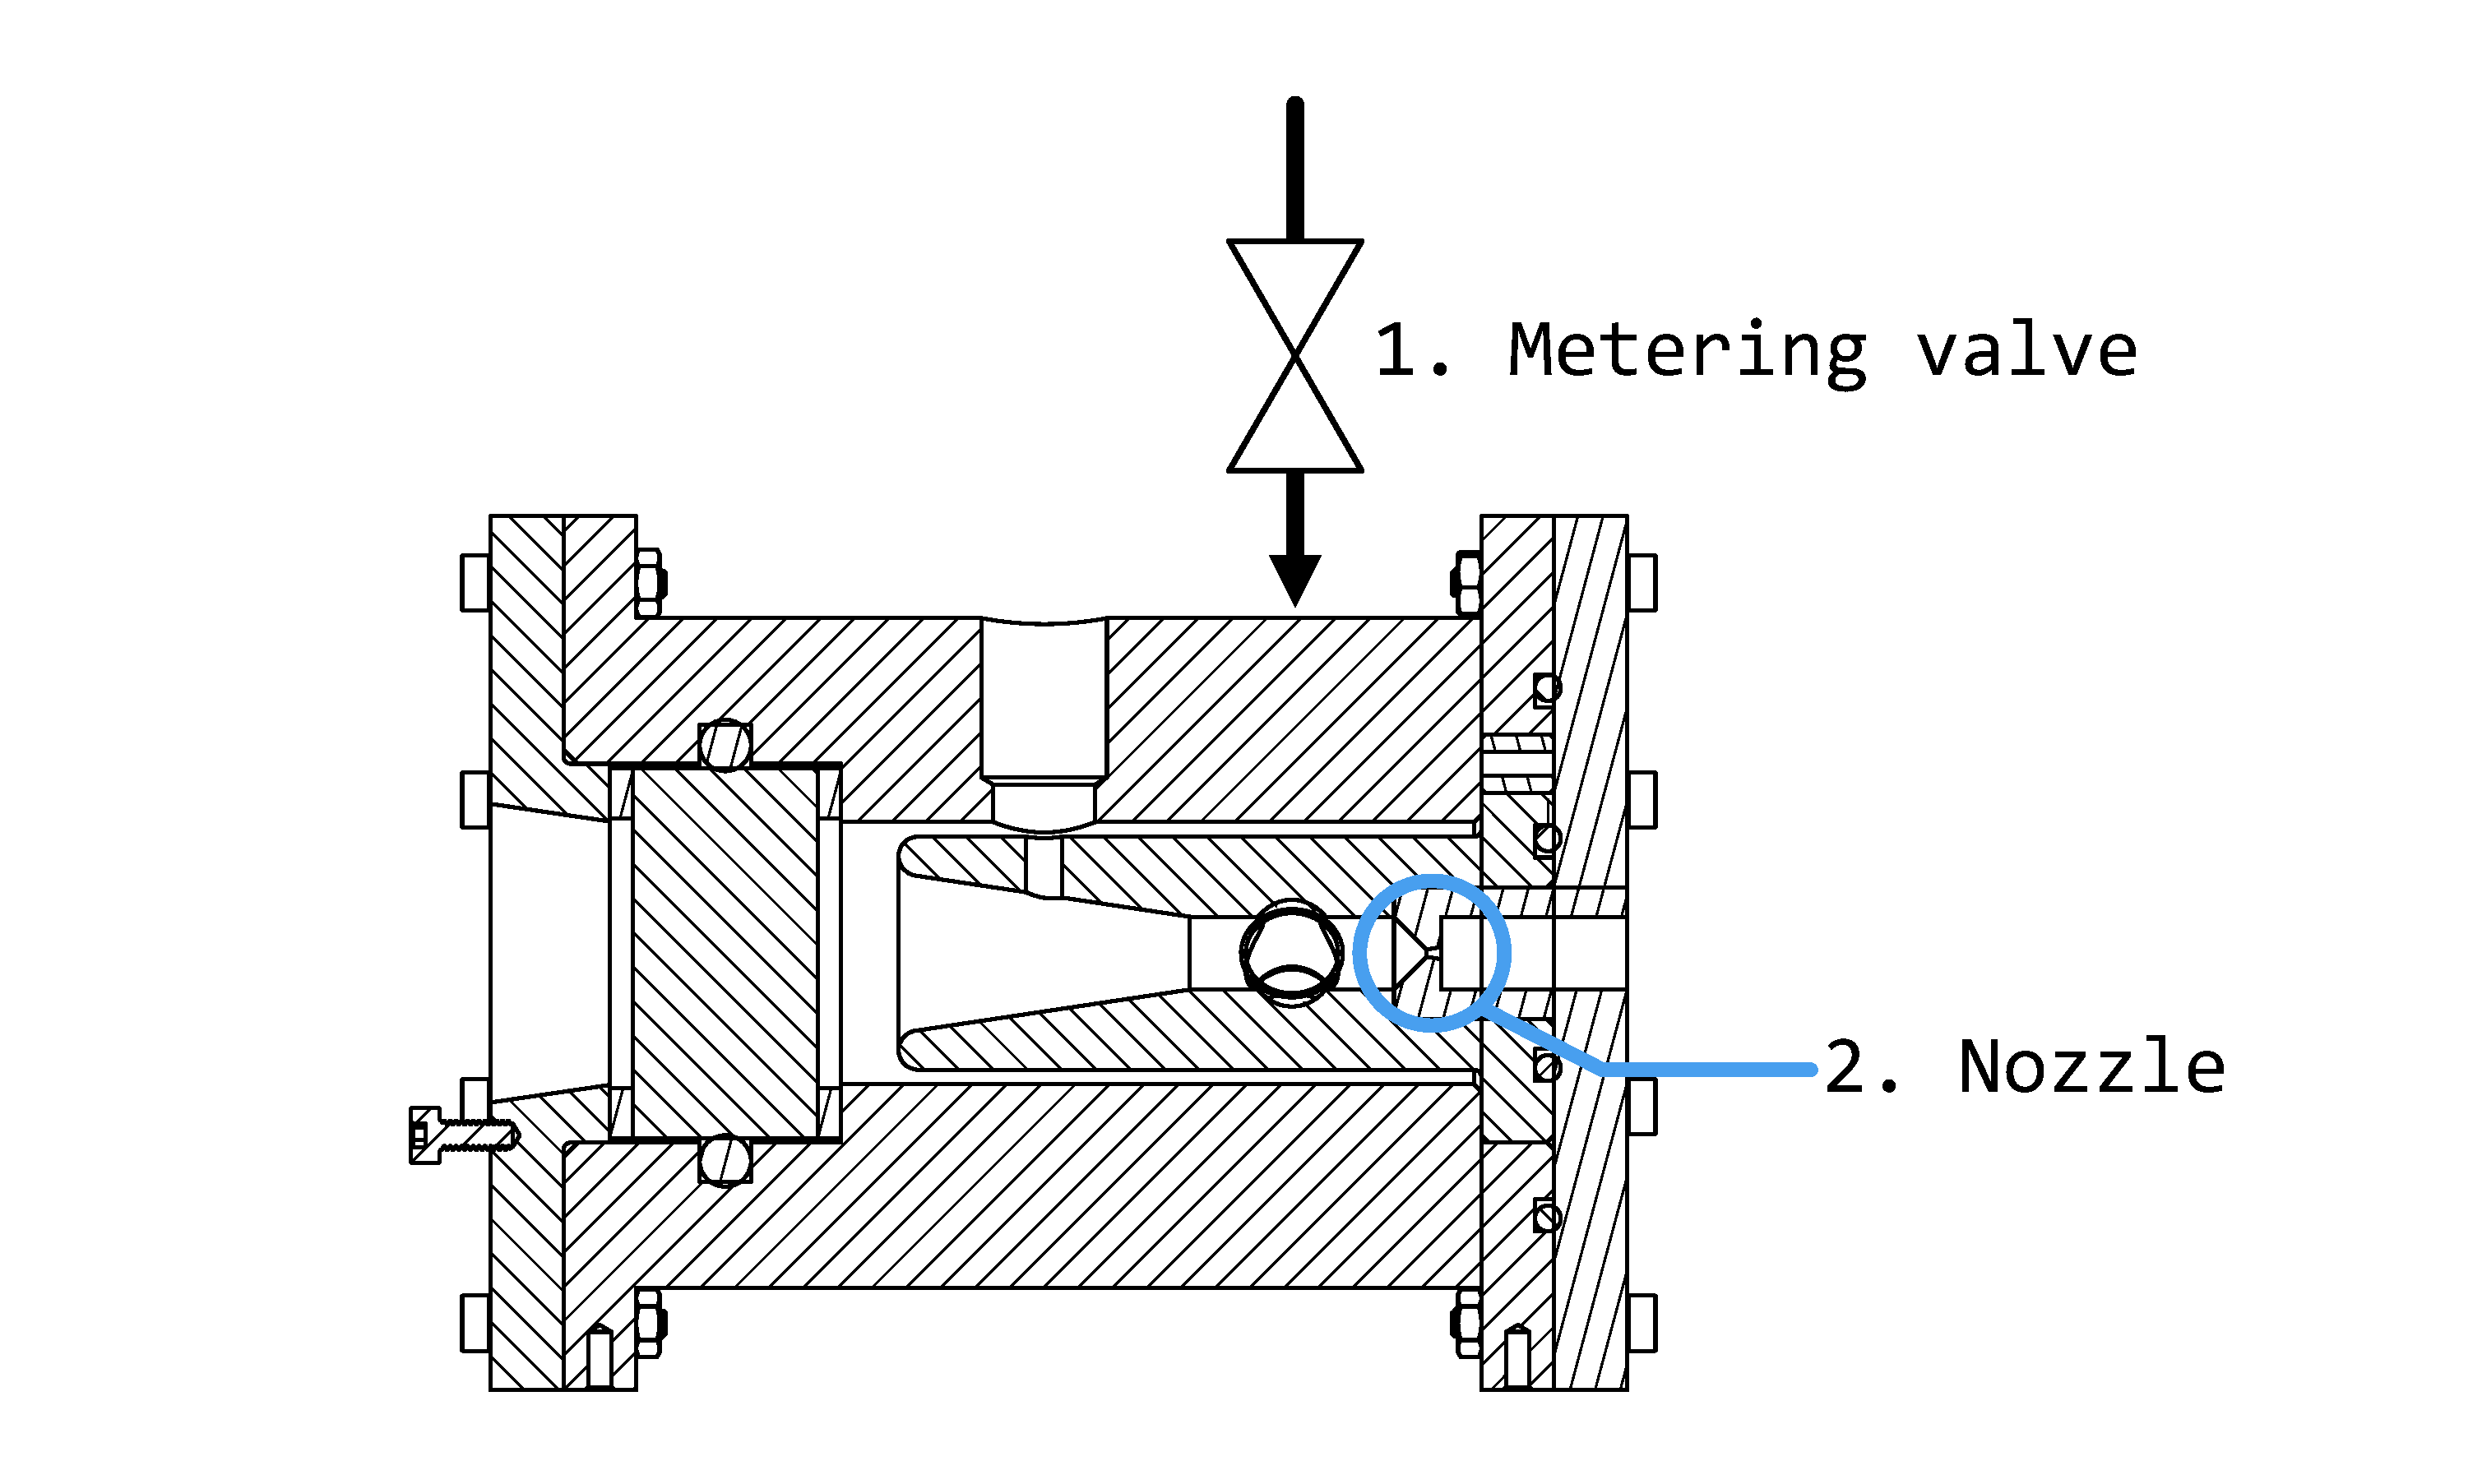
\includegraphics[width=0.8\linewidth]{assets/3 design/Double choked LTP thruster.pdf}
                \caption{Cutaway of a double choked LTP thruster showing both choking orifices: the metering valve and the nozzle.}
                \label{fig:double choke sizing}
            \end{figure}
            
            Starting with a cold gas thruster using argon, the speed of sound ($c_0$) is \qty{323}{m/s}. This is at ambient temperature (\qty{300}{K}), as we have no laser energy to heat the gas in this case. With a nozzle, the gas is accelerated to approximately twice this speed. The $v_\mathrm{exit}$, which is our main performance parameter, is therefore \qty{646}{m/s}.
            
            Laser on (hot) operation will now be examined. Taking the previous $v_\mathrm{exit}$ and ionizing the whole flow, it is posed that our efficiency is doubled. This gives a $v_\mathrm{exit}\approx \qty{1300}{m/s}$. What nozzle throat size is necessary for this $\dot m$ with $p_\mathrm{chamber} = \qty{25}{bar}$? We know that $\mathrm{MW_{Ar}} = \qty{40}{g/mol}$. The speed of sound is $c = \sqrt{\gamma R T}$. As we want to double the speed of sound, we are multiplying the temperature by 4.
            \[\text{Power} = \dot m (h_2-h_1)
            = \dot m c_p (T_2-T_1)\]
            Using a constant $c_p$ of argon of \qty{0.520}{kJ.kg^{-1}.K^{-1}}, the calculated $\dot m$ is \qty{0.641}{g/s}.
            
            Fliegner's formula describes the mass flow rate of an isentropic flow:
            \[\frac{\dot m}{A} = p_0\sqrt{\frac{\gamma}{T_0 R}}\frac{M}{(1+\frac{\gamma-1}{2}M^2)^{(\frac{\gamma+1}{2(\gamma-1)})}}\]
            With $\gamma = \frac{c_p}{c_v} = 1.666$ for argon and choked flow at the nozzle, the area and the diameter of the circular nozzle are \qty{0.176}{mm^2} and \qty{0.473}{mm}, respectively. These calculations can be repeated for the feed orifice, with the same $\dot m$, a pressure of \qty{50}{bar} and ambient temperature. This gives us an orifice size of about 0.2 mm.

            [COMPARED TO MEASURED, THIS IS MUCH SMALLER! WHY????]

        
        \section{V1 Spark initiation}
            
            As was discussed in \textcite{duplayArgonLaserPlasmaThruster2024a}, spark initiation was not reliable enough with the available electrode system. Opposing ports were drilled into the bottom of the apparatus to fit an electrode through the top and one through the bottom. This increased spatial repeatability of the spark and enabled the electrode gap length to be easily adjusted.

            In addition to this, the synchronization of the spark and the laser was found to be lacking. With the Photron high speed camera, the spark and the laser were separately imaged. The infrared laser being invisible to the camera, the beam was focused on one of the electrodes at low power. This caused the thin metal to glow white-hot when the laser is on. The following timings were determined by this investigation:

            \begin{figure}
                \centering
                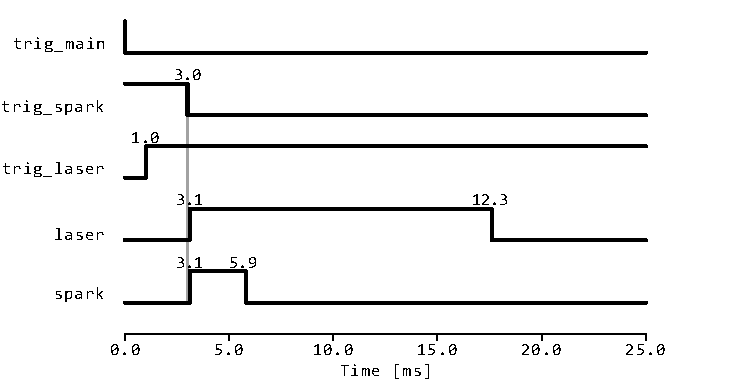
\includegraphics[width=\textwidth]{assets/4 experiments/timings.pdf}
                \caption{Signal timing diagram. The \textit{trig} prefix denotes triggering signals. The component is active when the line is high. Timings in \unit{ms} are also indicated on the figure.}
            \end{figure}

        \section{Electrodes}
            Static pressure testing up to \qty{75}{bar} for \qty{25}{minutes} was completed successfully. However, the off-the-shelf \qty{44}{kV} wire originally intended to be used as the electrodes burst during pressure tests. An electrode redesign was therefore necessary. Molded dielectric epoxy (Stycast ES 1001 [LINK to website]) around an industrial sewing needle core was chosen, as it was economical and the outer diameter of the electrodes could be precisely controlled by sanding the surface of the set epoxy. Molds were 3d printed and Mann Ease Release\texttrademark 300 was applied to all their inside surfaces.

            \begin{figure}[!ht]
                \centering
                \begin{subfigure}[t]{0.30\textwidth}
                    \centering
                    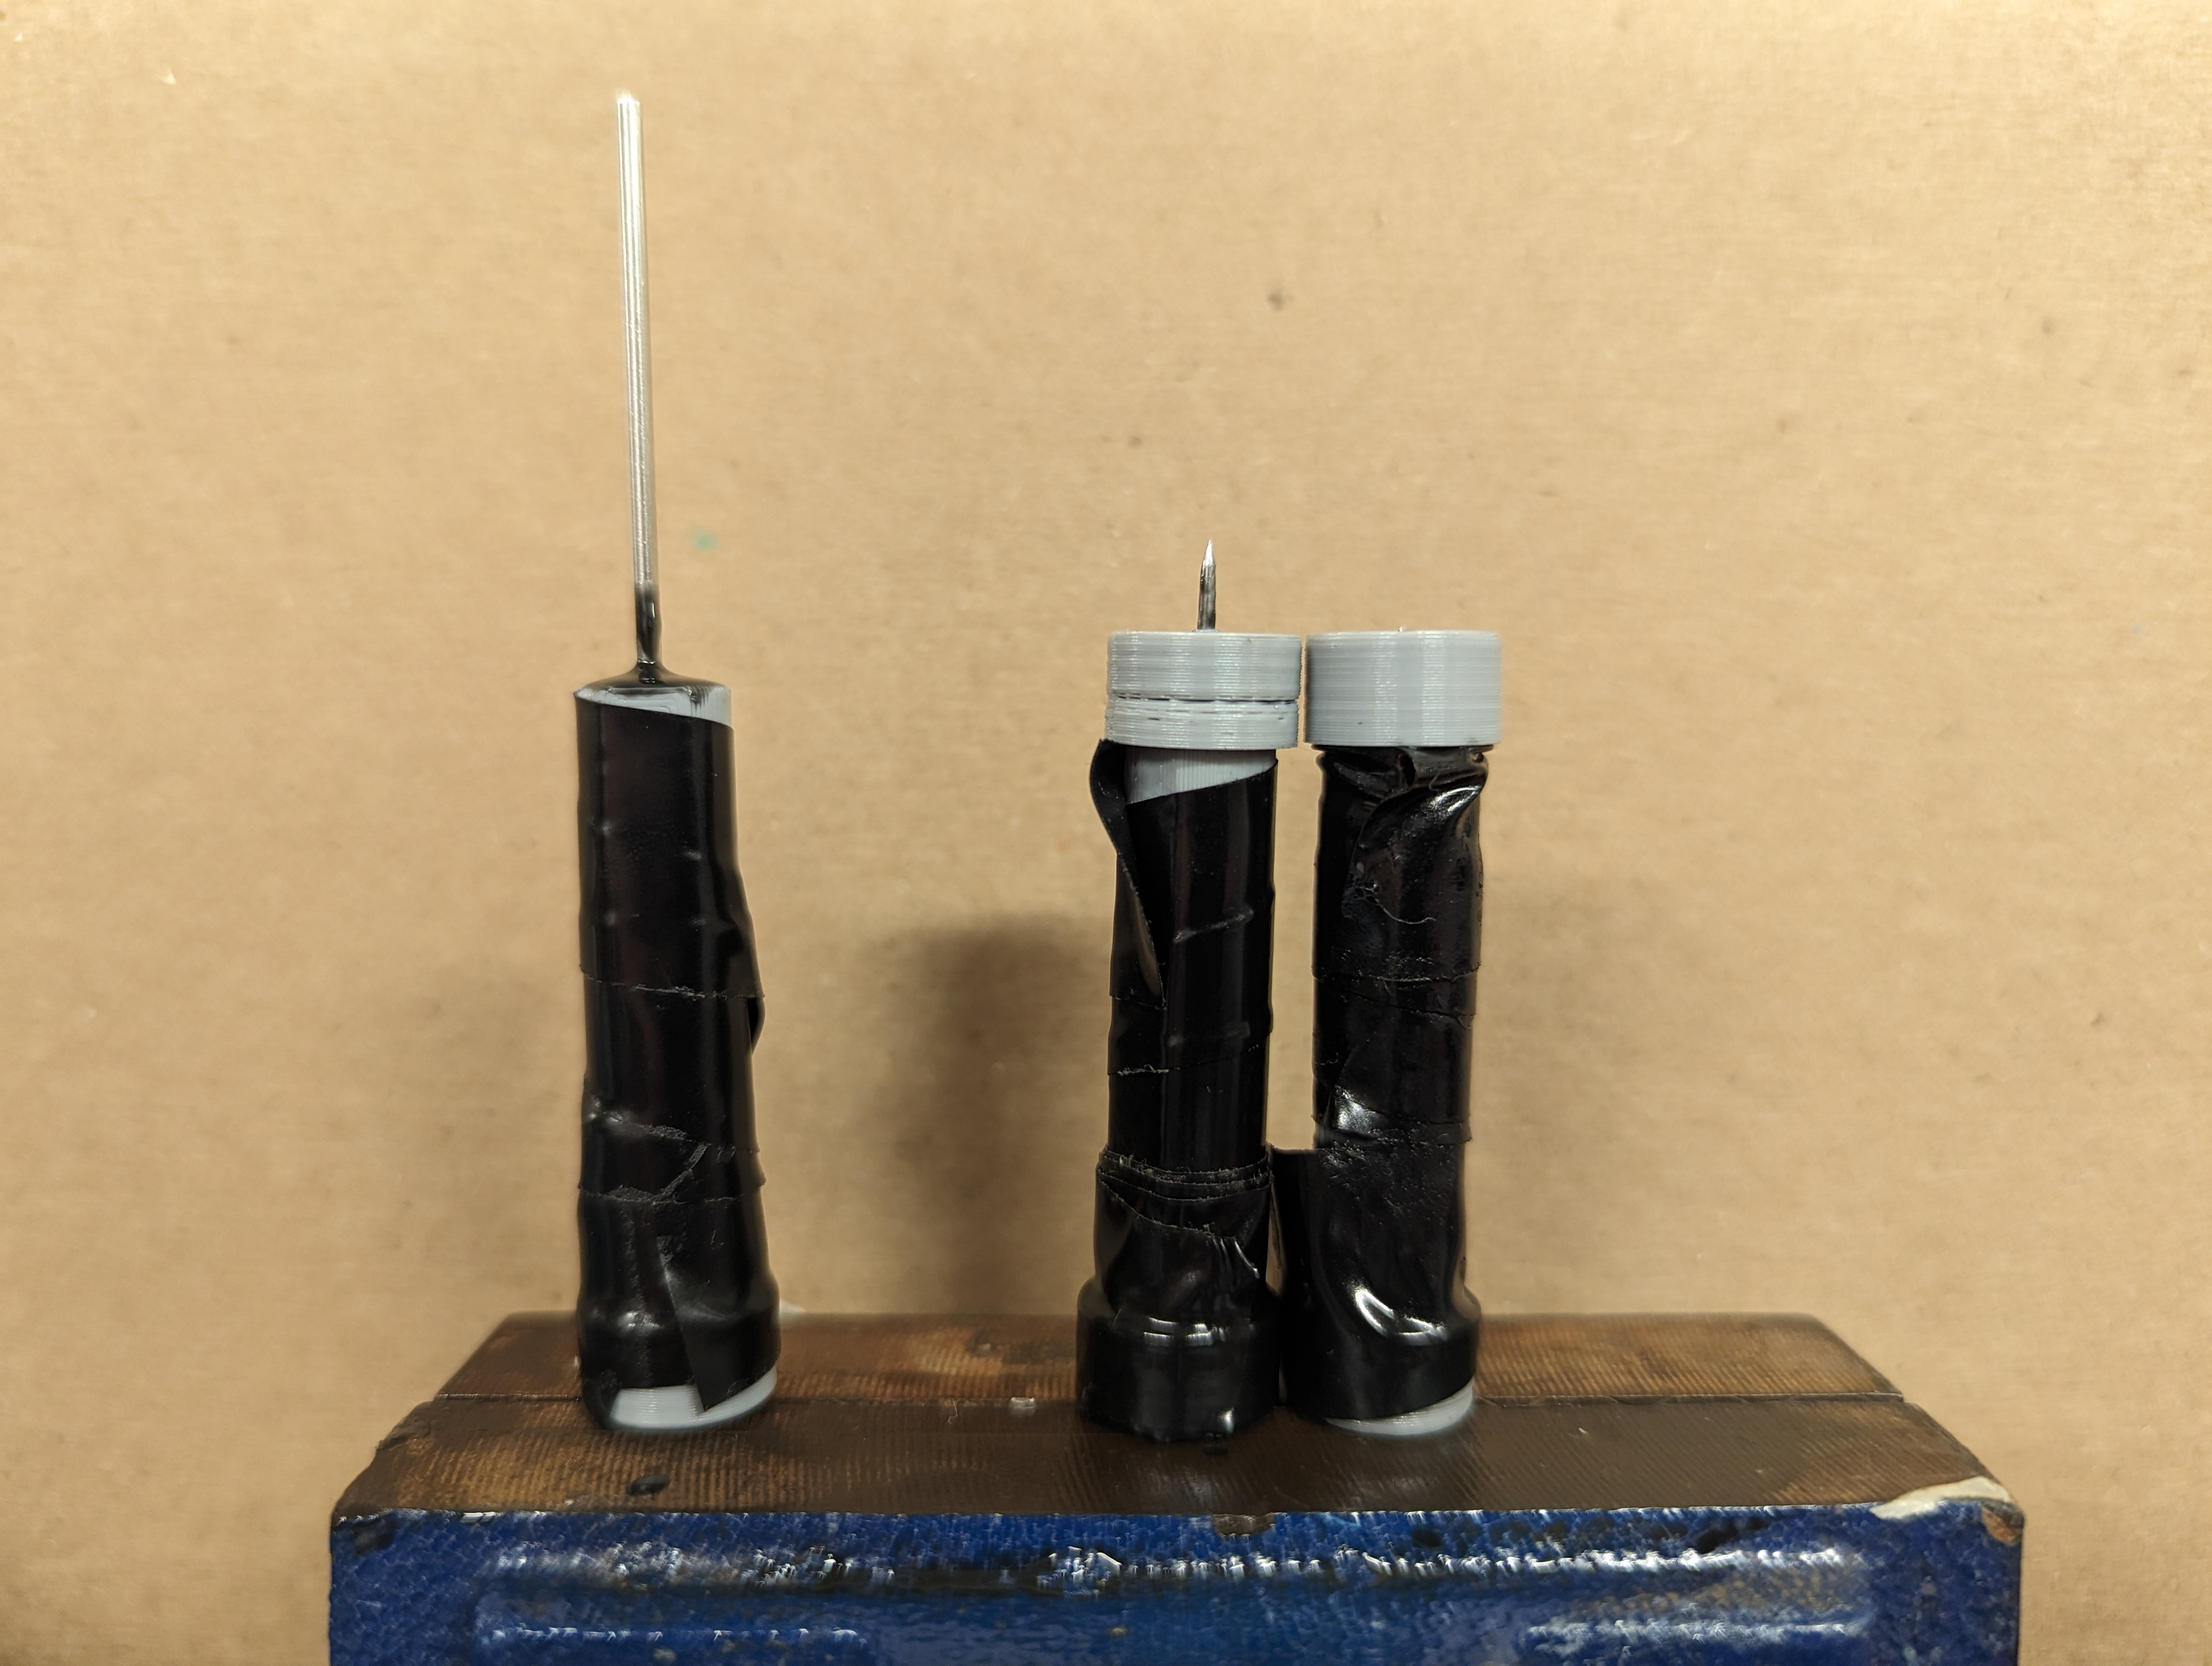
\includegraphics[width=\textwidth]{assets/3 design/Molds.jpg}
                    \caption{Molds with steel needle core in place}
                \end{subfigure}
                \hfill
                \begin{subfigure}[t]{0.30\textwidth}
                    \centering
                    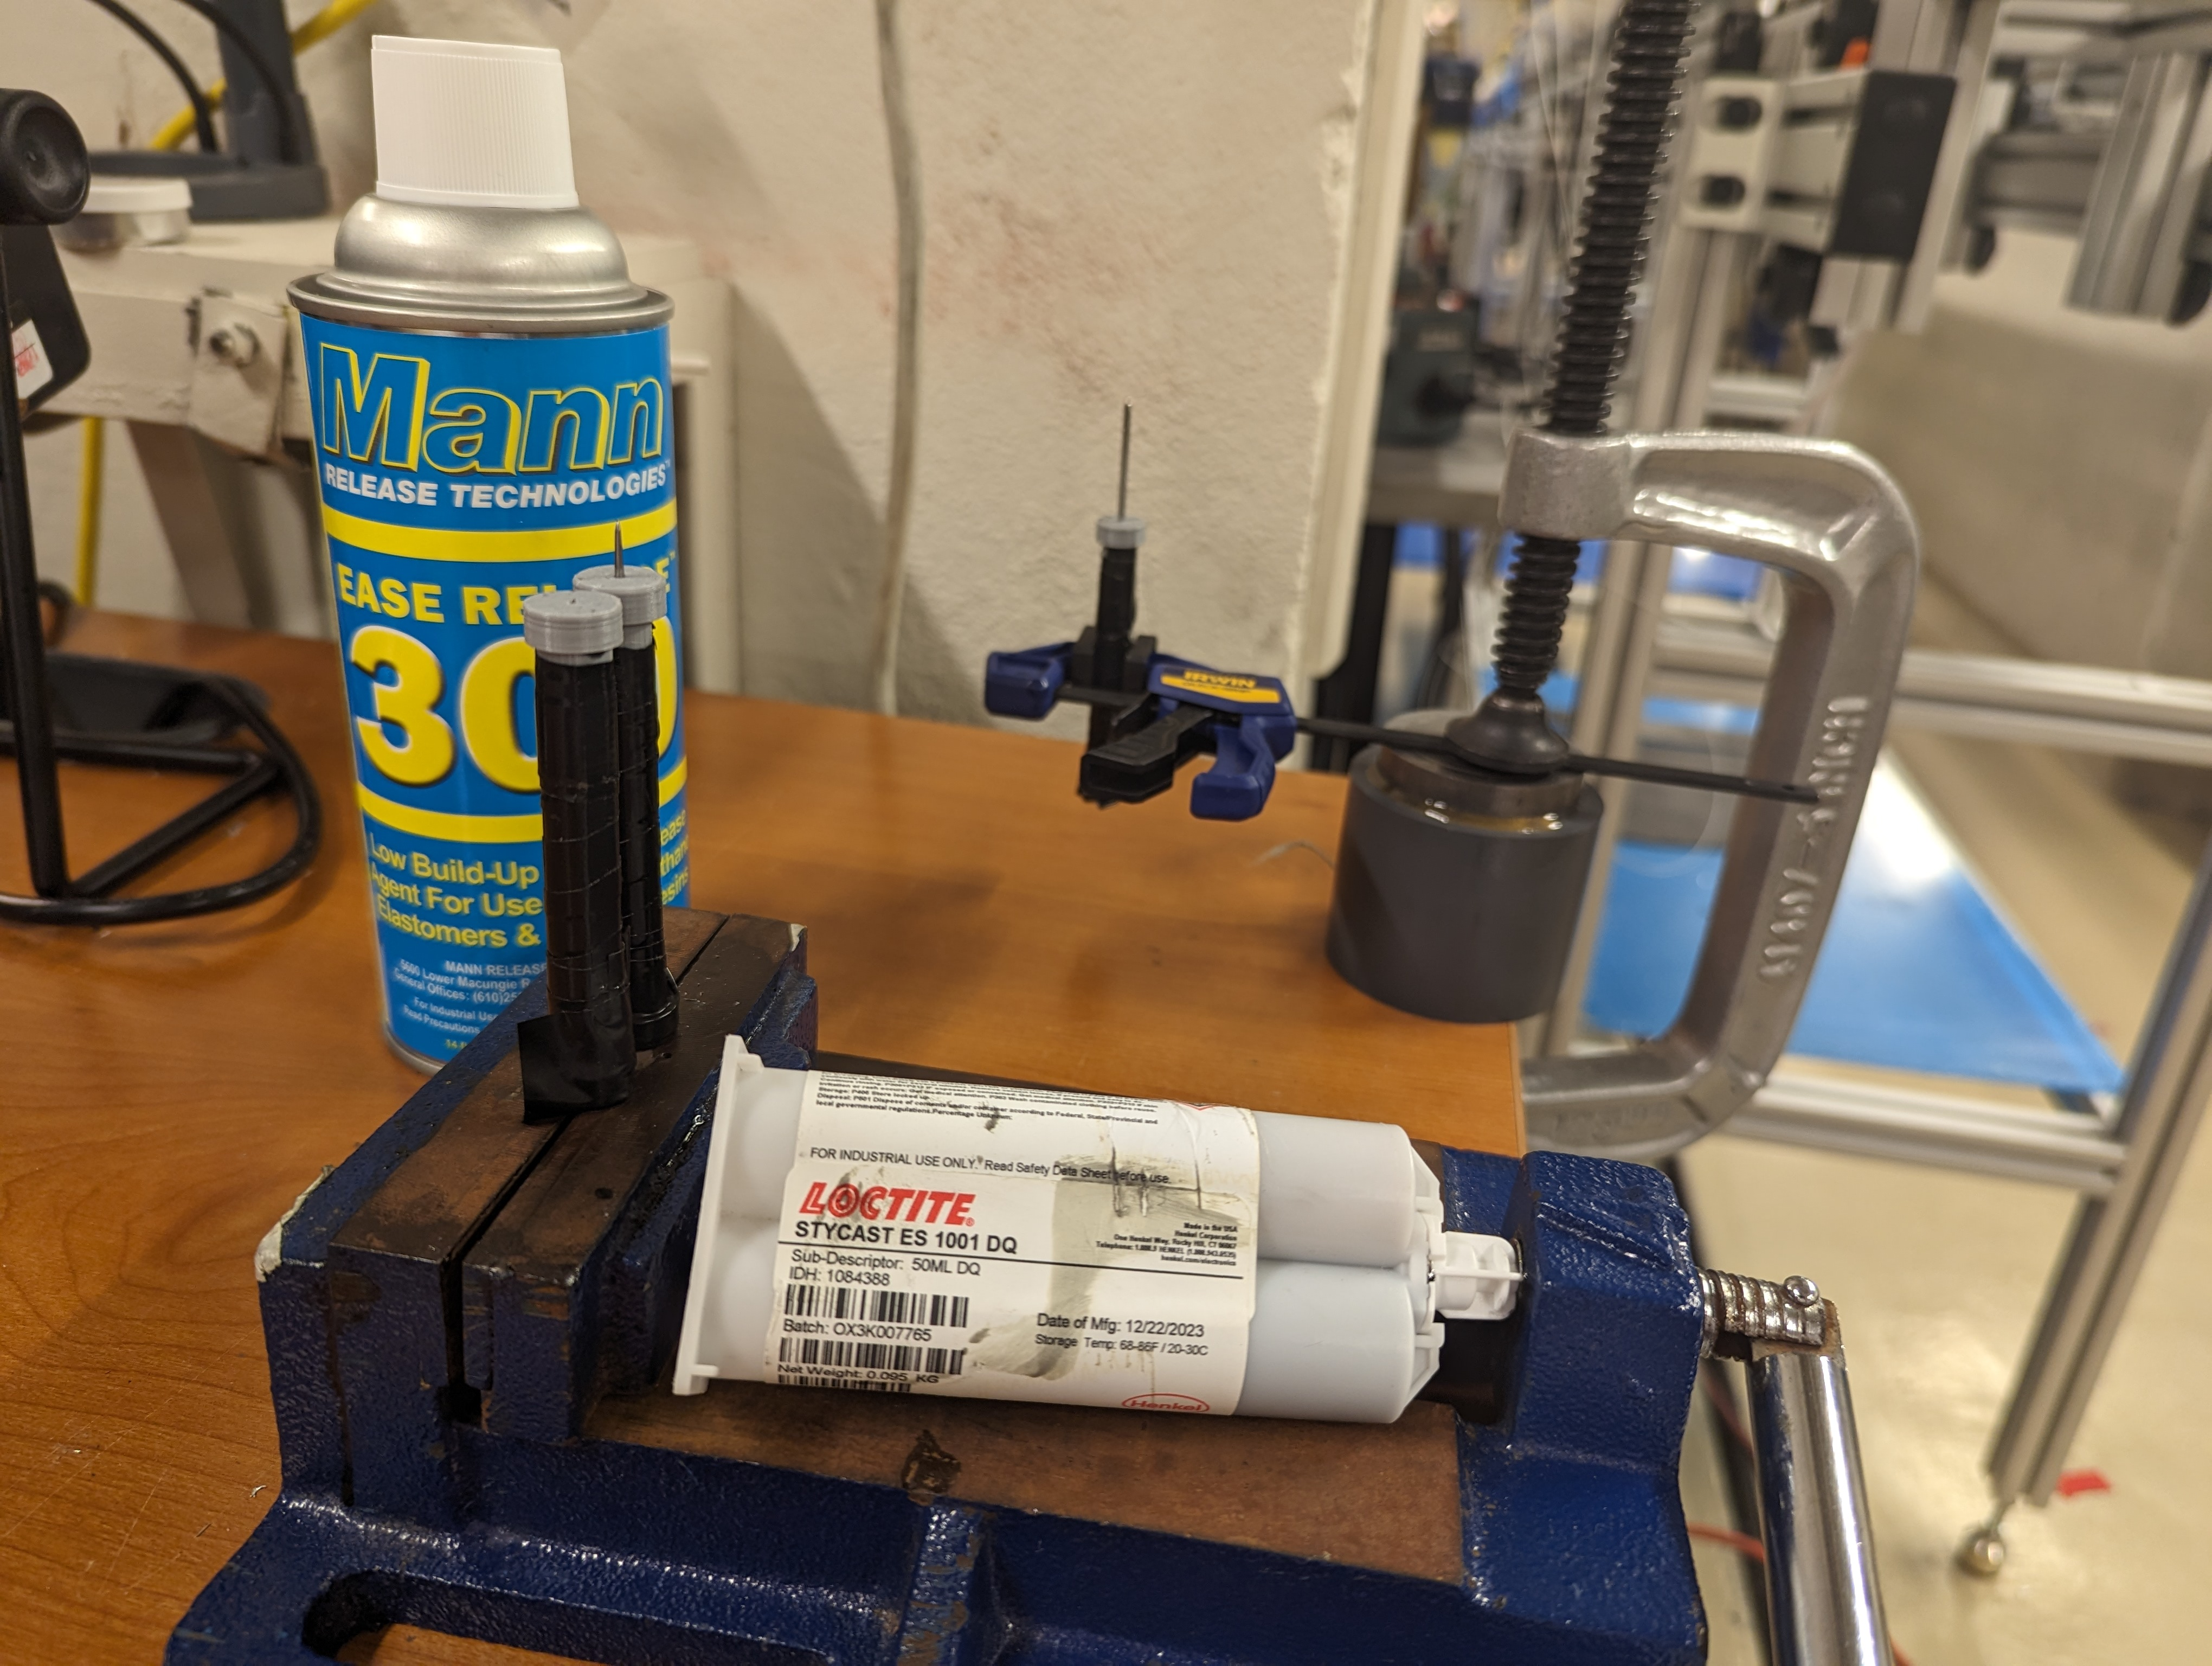
\includegraphics[width=\textwidth]{assets/3 design/Mold process.jpg}
                    \caption{Molding process}
                \end{subfigure}
                \hfill
                \begin{subfigure}[t]{0.30\textwidth}
                    \centering
                    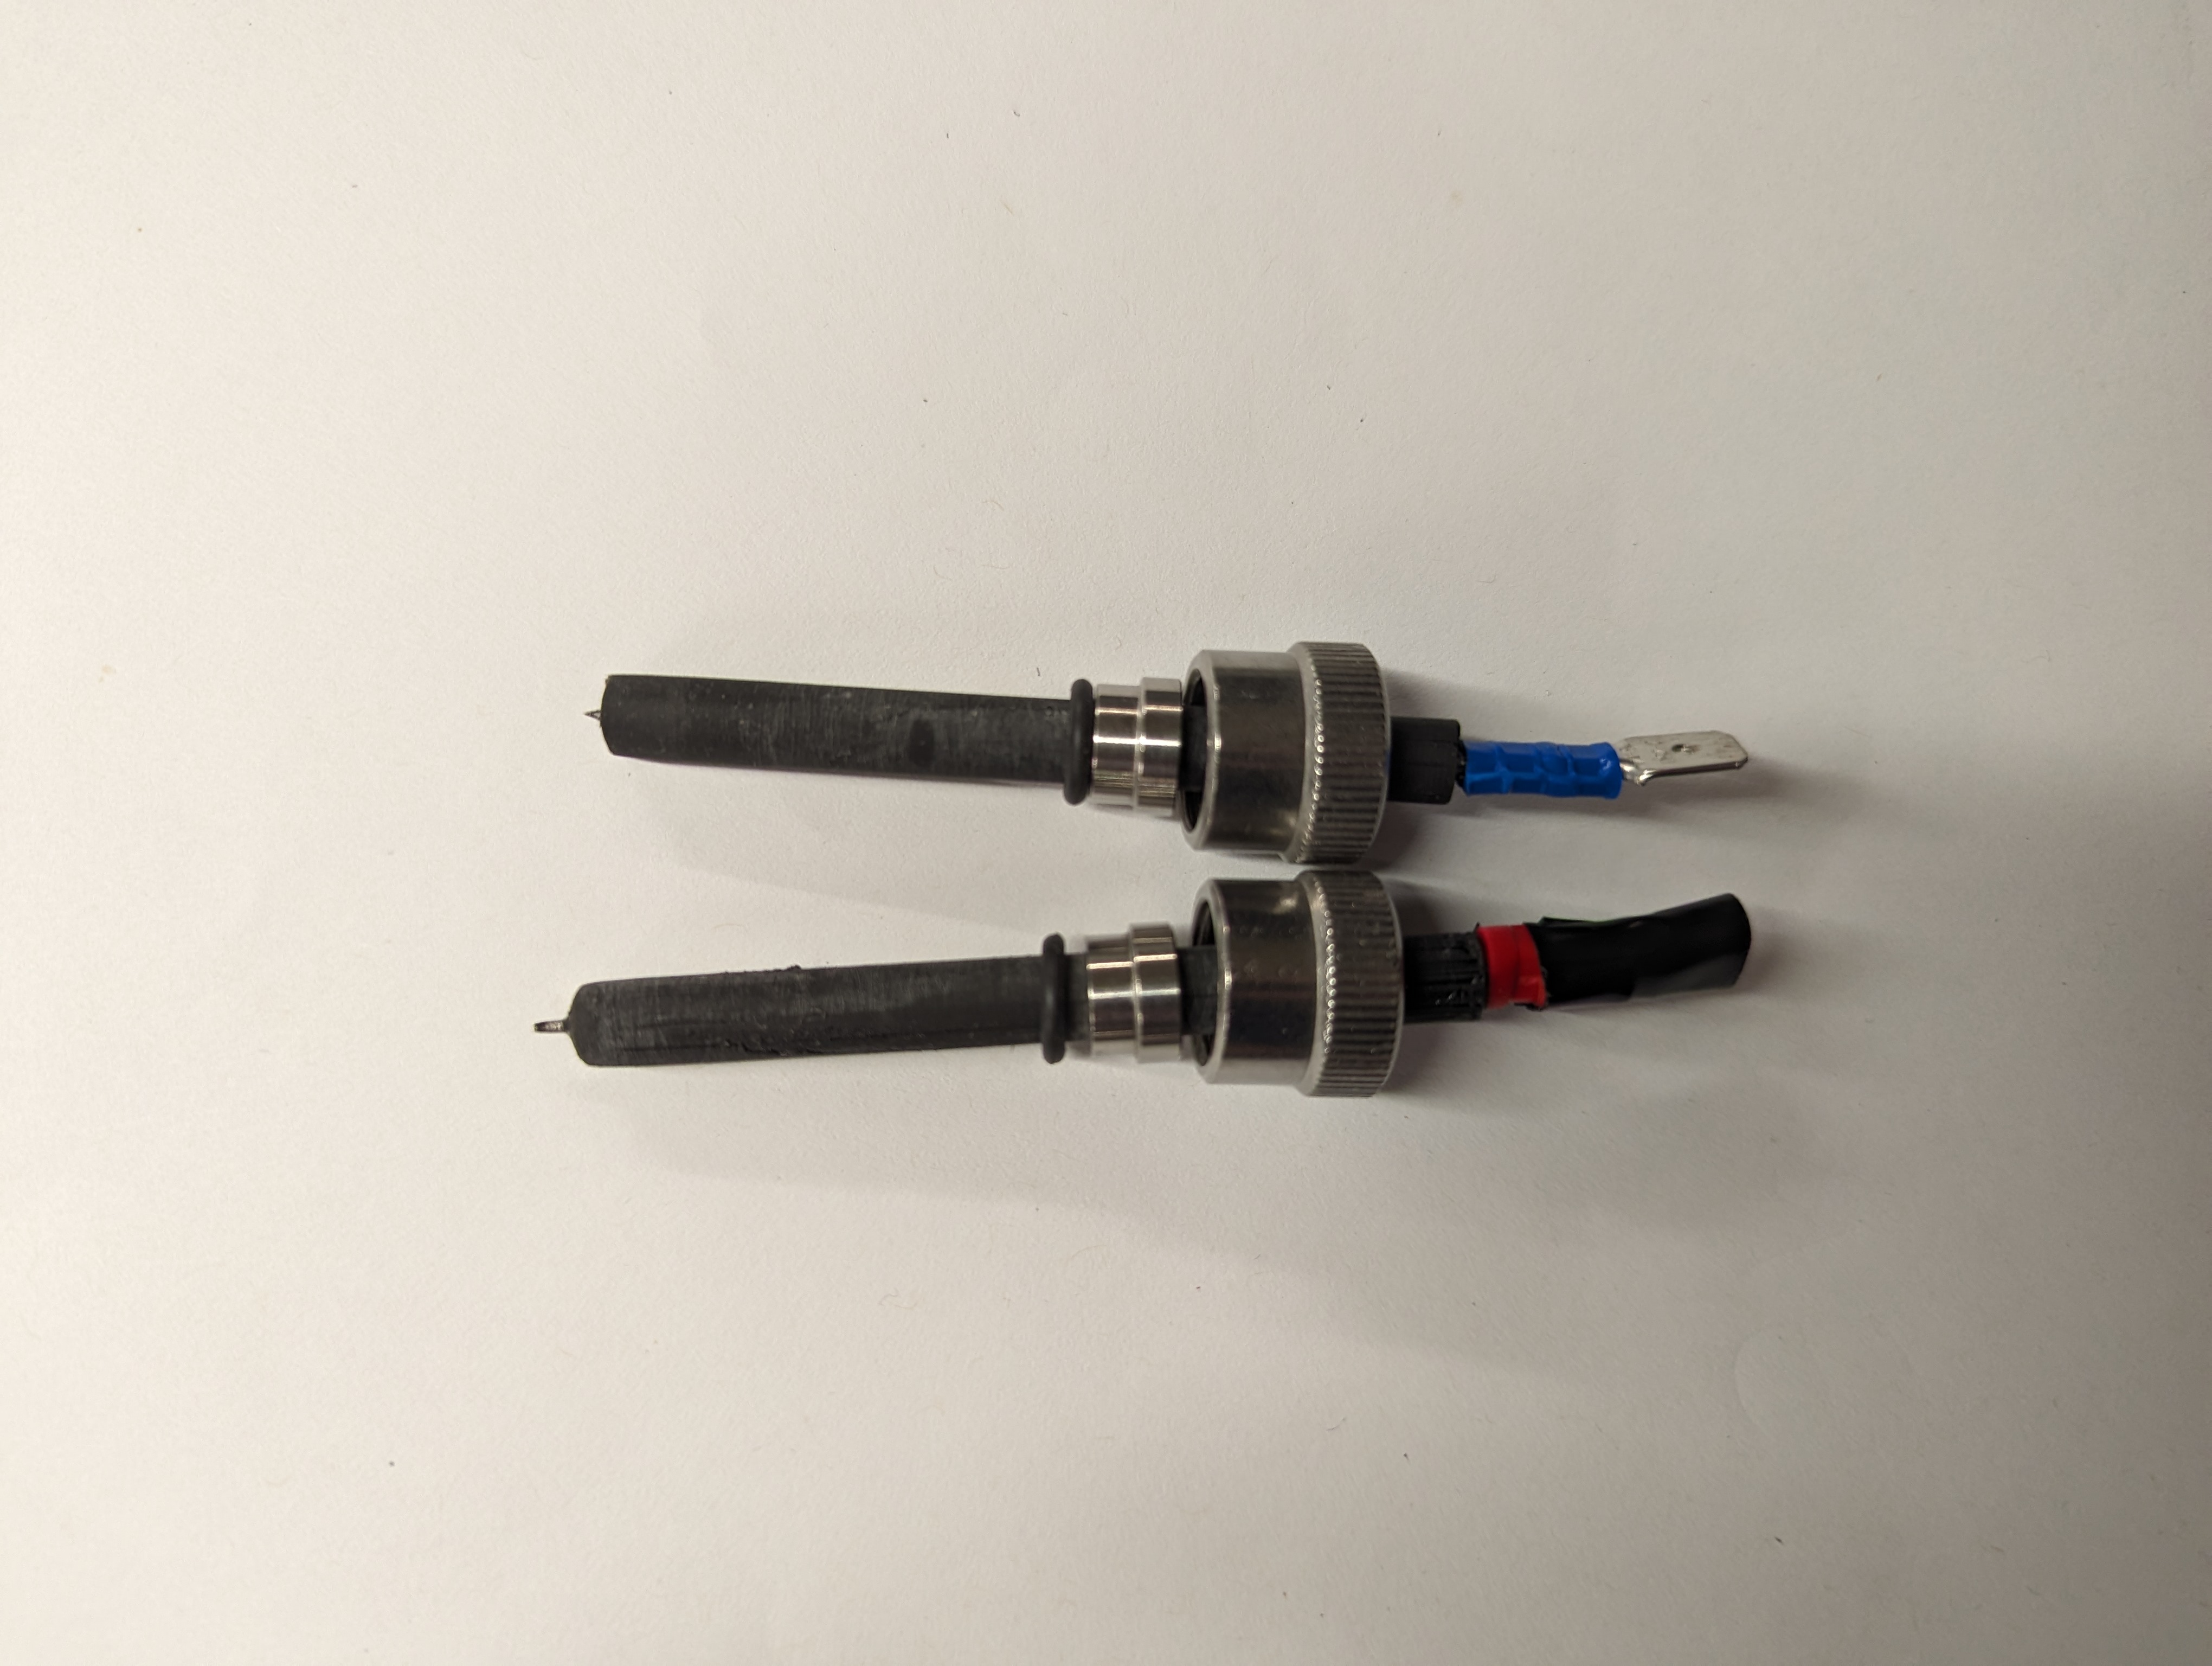
\includegraphics[width=\textwidth]{assets/3 design/V2 electrodes.jpg}
                    \caption{Assembled electrodes with Ultra-Torr cap and electrical connectors}
                    \label{fig:Assembled electrode}
                \end{subfigure}

                \caption{Electrode manufacturing process}
            \end{figure}

            The electrodes were then sanded down to fit tightly into Ultra-Torr vacuum connectors [link to swagelok and part number]. Although these connectors were not designed for high pressure, previous experience has shown that they are appropriate up to about \qty{20}{bar} of internal pressure if tightened enough.

            The result is presented in \autoref{fig:Assembled electrode}.

            Once installed in the V2 thruster, the electrodes were pushed into contact with each other and the Ultra-Torr connectors tightened. Statically pressurizing V2 to \qty{20}{bar} was enough to slightly separate the electrodes from one another. [add text for flow testing?]

            \section{Optics design}
                
                Due to the low continuous laser power compared to experiments in the literature, increasing the laser flux with small a focus is critical.

                Two ways can be used to calculate the spot size of a laser. Firstly, ray tracing software such as WinLens calculate the geometry of paraxial \footnote{Rays having small angles and distances to the optical axis} rays and show the path of these rays at the focus. Secondly, this equation \cite{LaserSpotSize} can be used: (ideal?)
                
                \[
                \text{Spot size}(mm) = \frac{4 \times \text{Focal length}(mm) \times \text{Wavelength}(mm) \times M^2}{\pi \times \text{Beam diameter at lens}(mm)}
                \]

                The beam propagation factor $M^2$ is a scale to measure beam quality. A diffraction-limited Gaussian beam has the minimum $M^2$ of 1 \cite{hechtUnderstandingLasersEntry2019}. 
                
                The YLR-300/3000 laser has a BPP of \qty{2}{mm.mrad} [Refer to appendix laser's data sheet].

                
                
                It is also implemented in WinLens, but is not based on ray tracing.

                The following spot diagrams were produced with WinLens. Note the difference in scales and spacing used throughout.

            

                \begin{table}[!ht]
                    \centering
                    \caption{Simulated focal length and spot diameter of various lens assemblies in WinLens3D. Laser flux is also calculated for \qty{300}{W} of incident power}
                    \label{tab:laser flux}
                    \begin{tabularx}{\textwidth}{@{}lX<{\raggedright}X<{\raggedright}X<{\raggedright}X<{\raggedright}@{}}
                    \toprule
                    Lens & Nominal focal length (\unit{mm}) & Focal length at \qty{1070}{nm} (\unit{mm})& Beam diameter at focus (\unit{mm}) & Laser flux at \qty{300}{W} (\unit{W/cm^2}) \\ \midrule
                    Single & 125           &  122   &    0.0863 ?  0.20?     &  \\
                    Single & 100           &  93   &    0.20   &  \\
                    Double & 500, 150      &  110    &    0.08   &  \\
                    \bottomrule
                    \end{tabularx}
                \end{table}

                (Maybe compare with minimum maintenance intensity of previous literature)

                In a two element system, the longest focal length lens should be placed first, as the diameter of the beam entering the second lens is maximized. However, it is placed after here because it is impossible to mount before. The difference in spot size is acceptable. [maybe compare?]

                Practical considerations for experiments are the following. When aligning the laser with the red visible guide beam, chromatic abberations [\dots] \cite{hechtUnderstandingLasersEntry2019}.

                The LSP will also be formed upstream of the laser focus when there is no gas flow. Therefore, the focus needs to be slightly after the ignition system. [does this change with flowing LSP?]

                \subsection{CW power test}

                Wanted to see where exactly the pulsed power threshold was. For this, needed a max CW power measurement to compare against. 
    
                Tried to measure max CW power through two lenses, without the V2 apparatus. The two lenses were rated for this flux, but the 500 mm focal length lens shattered after about \qty{50}{s} of CW lasing. The leading hypothesis is that as the lens' temperature increased, it expanded, shattering it
    
                [graph of laser power that broke lens]
    
                \begin{figure}[!ht]
                    \centering
                    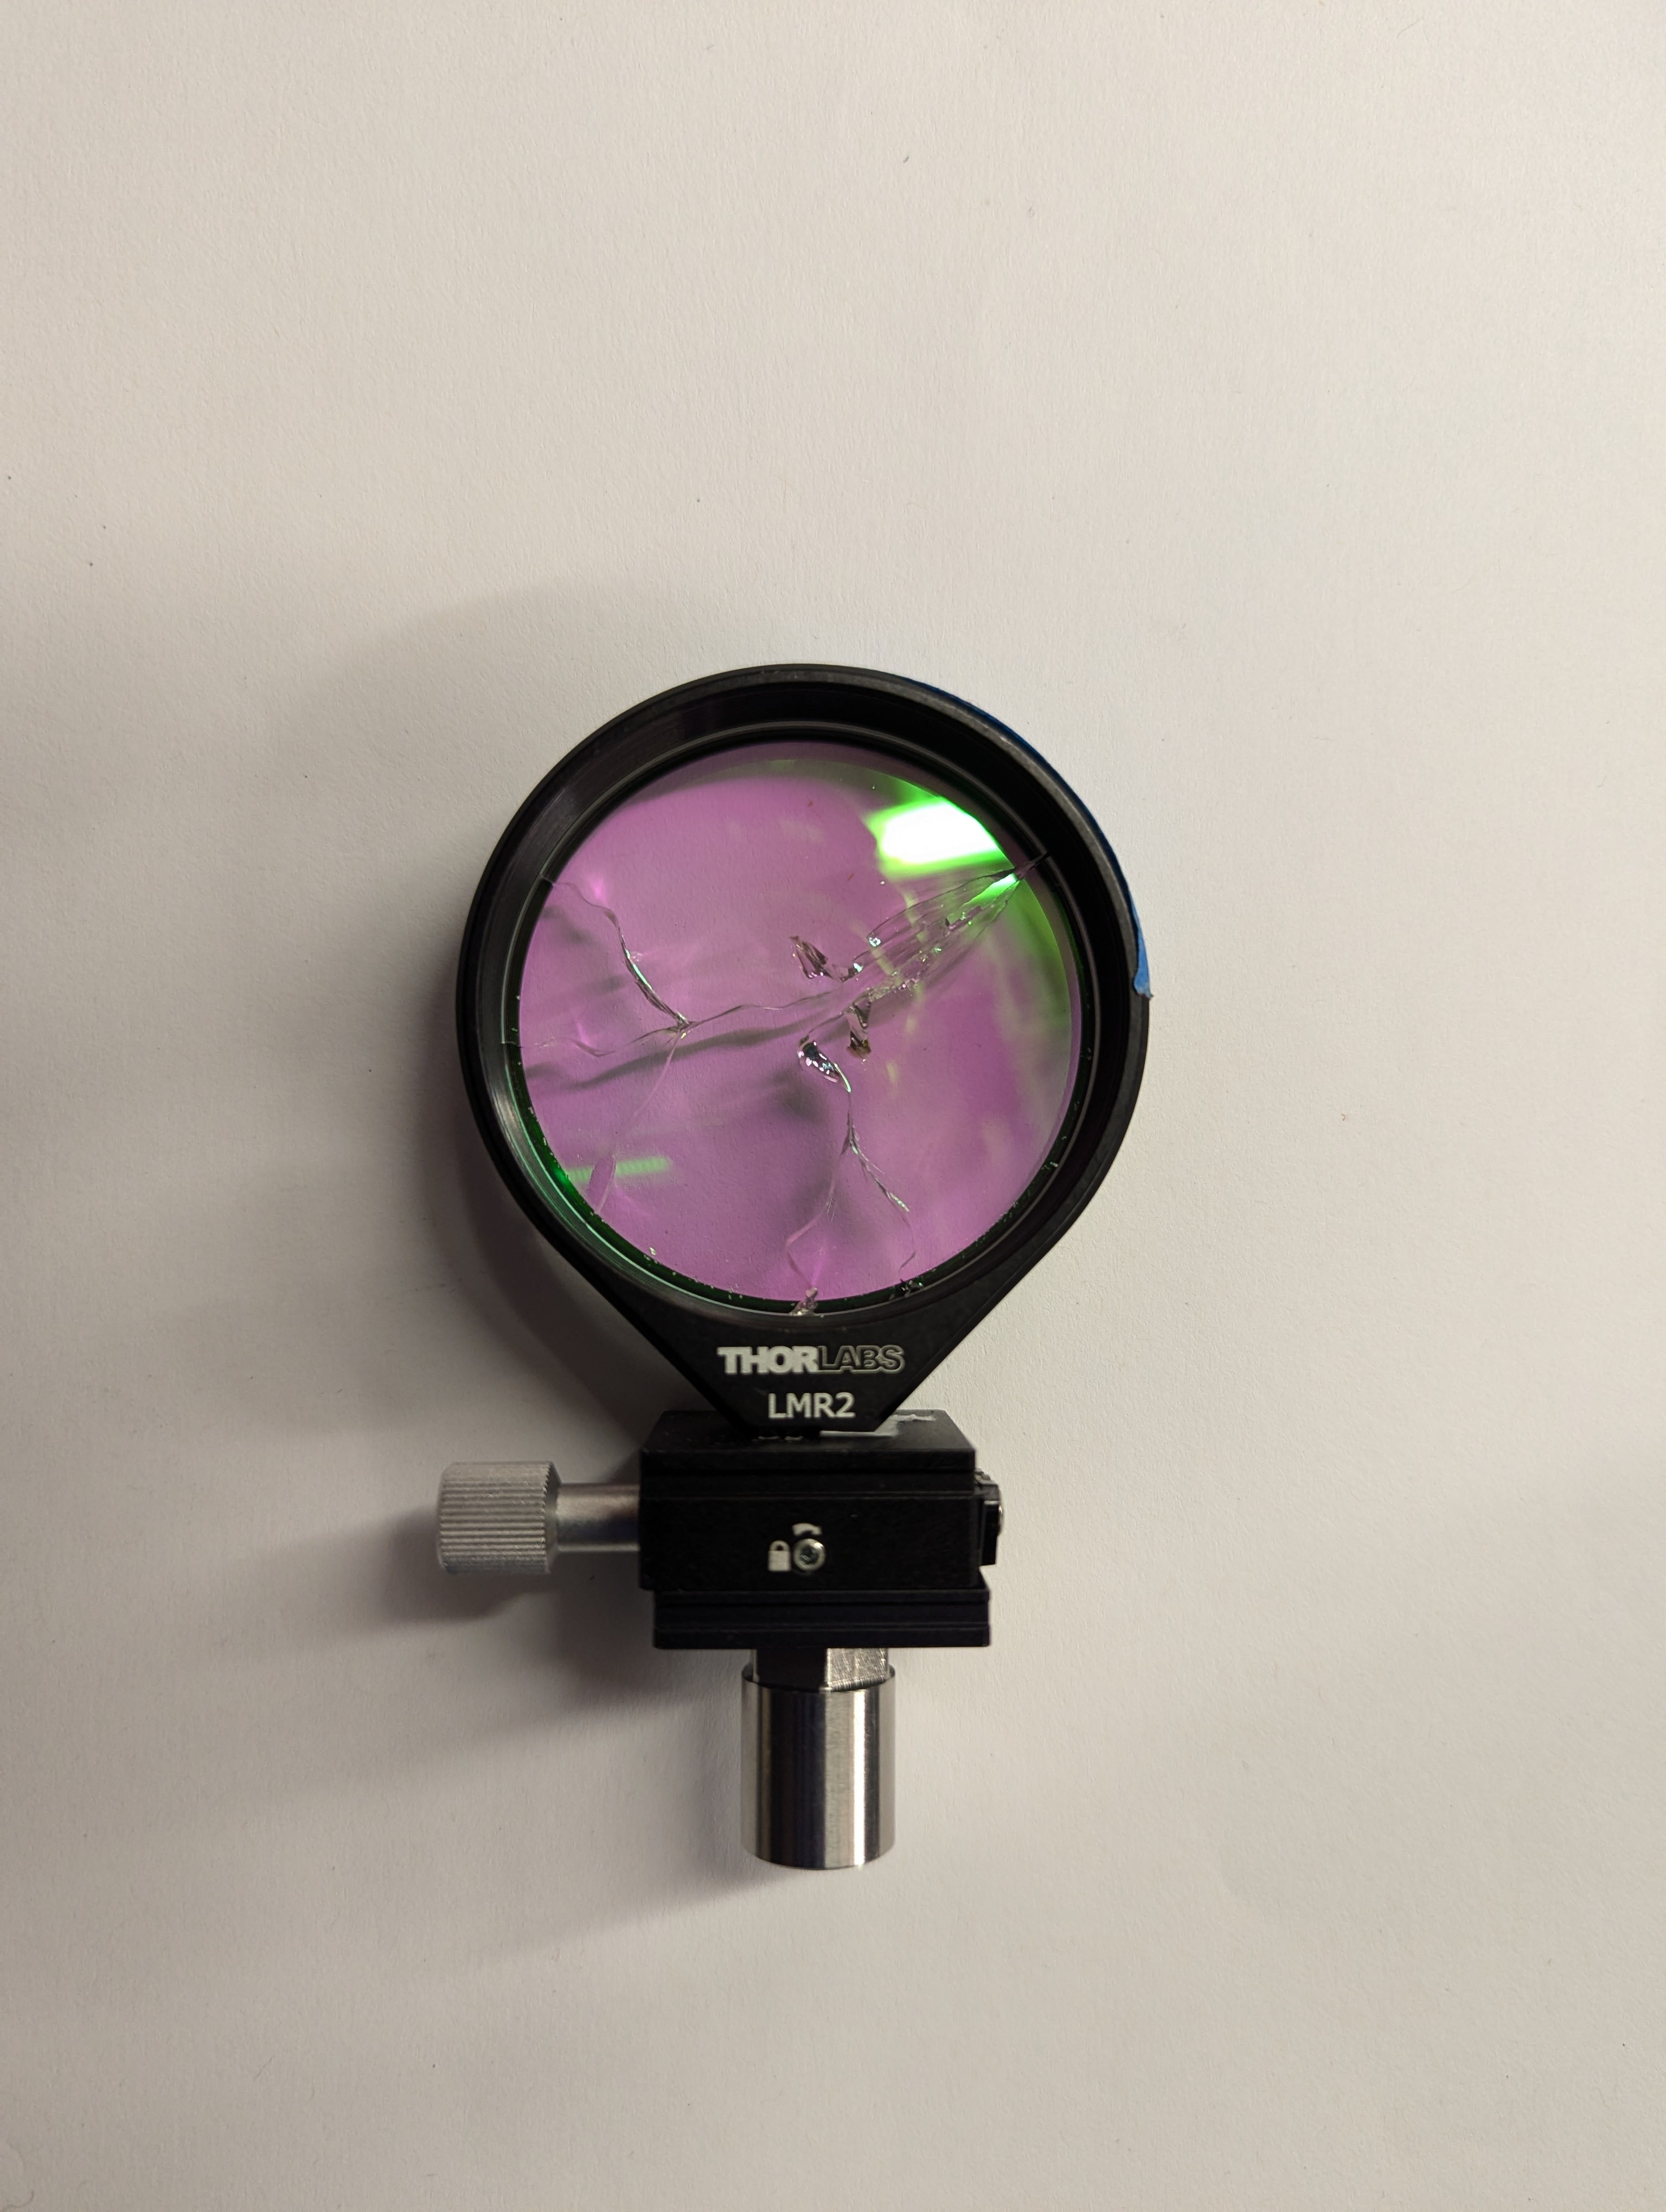
\includegraphics[width=0.5\textwidth]{assets/4 experiments/Shattered 500 mm lens.jpg}
                    \caption{Shattered 500 mm lens}
                \end{figure}
    
                This test showed a \qty{316}{W} (?) max CW power.
    
                Therefore, future CW tests will have to stay under this maximum time period, unless a lens cooling system is implemented. This could be as simple as a fan blowing cool air onto the lens.

            \section{V1 Bringing the pulsed power down and optical design} \label{sec:pulse_power_down_V1}
            
                Pulsed shots at lower power levels revealed a difficulty to initiate the LSP below \qty{20}{\%} power, which corresponds to about \qty{620}{W}. This poses a problem, as the maximum CW power of the laser is significantly lower, at \qty{350}{W}. A test campaign was started in February 2024 to determine if LSP initiation in the V1 thruster was possible under this maximum CW power level.
                
                To obtain LSP initiation, a high enough laser flux is needed. With a fixed power, it is necessary to focus the laser down to the smallest area possible to get the highest flux. Quantifying the diameter of this focus was therefore the first step. 
    
                %Section on quantifying diameter, laser optics basics (email from thorlabs guy)
    
                For a multi-element system, the spot diameter must be calculated numerically with ray tracing software. WinLens 3D Basic \cite{QioptiqQShopFree} was used here, as it is free and powerful enough for this application. The single element system was also simulated in this software to verify the calculations.
    
                Now that the diameter of the focus is known, two avenues are possible to improve it: a shorter focal length or a multi-lens system \cite{LensTutorial}. At first, a single lens with a \qty{125}{mm} focal length (Thorlabs LA1384-C [CITE 125mm lens]) was used, as it was the simpler option. During these shots, the goal was to achieve LSP initiation at or below \qty{11}{\%} pulsed power, or \qty{340}{W}. The following graph shows LSP initiation attempts at various power settings and axial lens positions. 20 pulsed laser shots were performed for each point on the graph. If at least one was successful at igniting LSP, it was recorded as such. This graph can also be interpreted as a beam profiling for LSP conditions.
                
                % Graph of 125mm lens
                \begin{figure}[!ht]
                    \centering
                    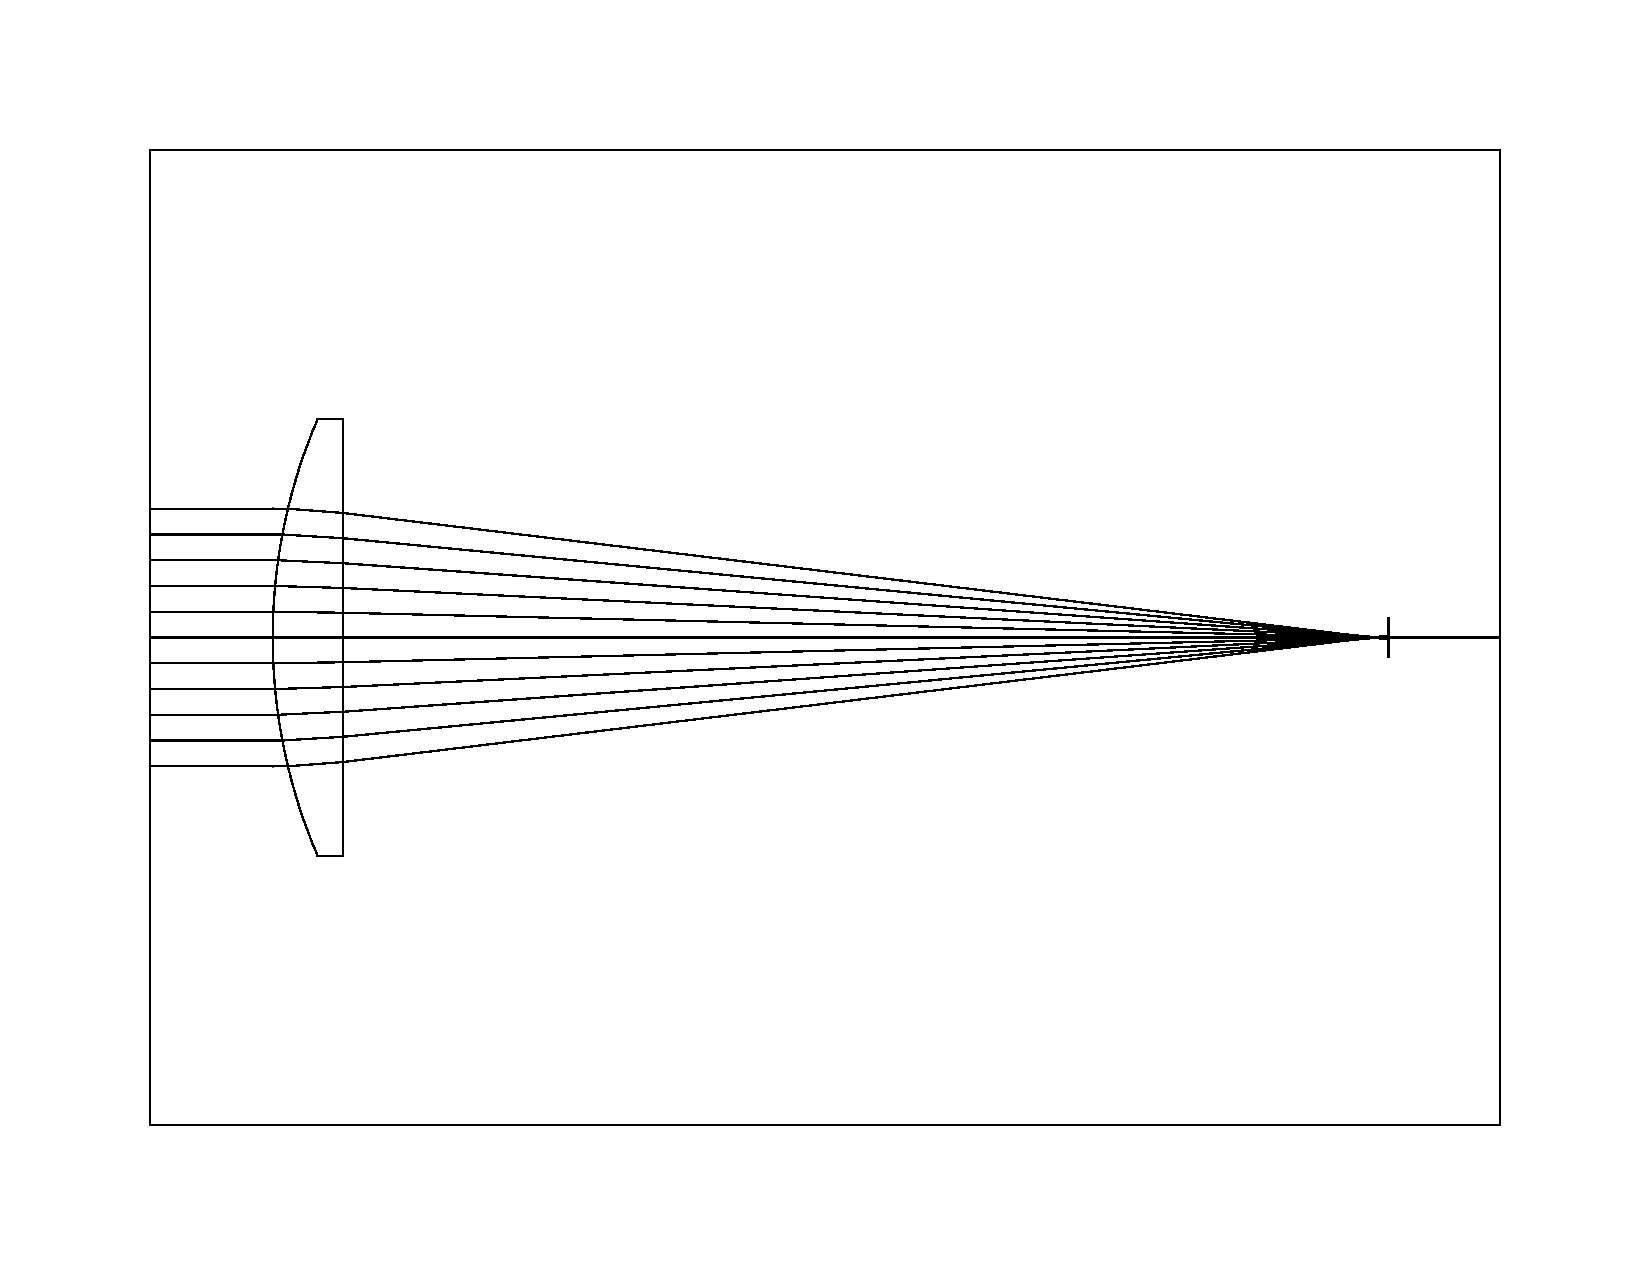
\includegraphics[width=\textwidth]{assets/4 experiments/125lens.pdf}
                    \caption{125 mm focal length lens}
                \end{figure}
    
                \begin{figure}[!ht]
                    \centering
                    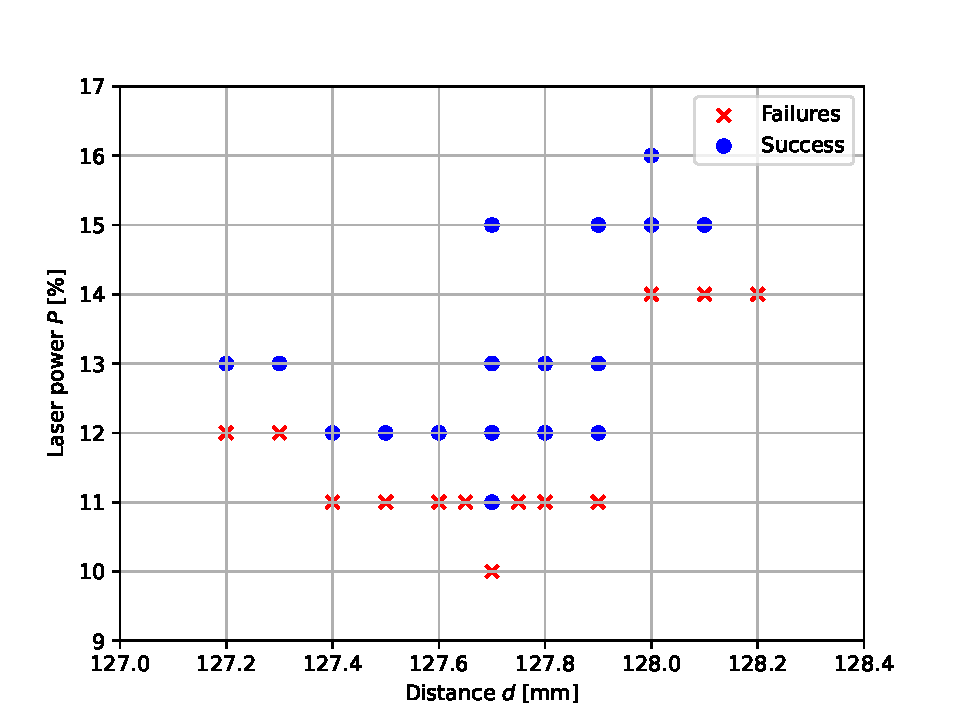
\includegraphics[width=0.75\textwidth]{assets/4 experiments/125mm_focus_threshold.pdf}
                    \caption{125 mm focal length lens}
                \end{figure}
                
                Initiation at \qty{11}{\%} was attained once, but it was not possible to replicate this. A tighter focus was necessary to increase initiation reliability.
    
                % Graph of multi-lens
                \begin{figure}[!ht]
                    \centering
                    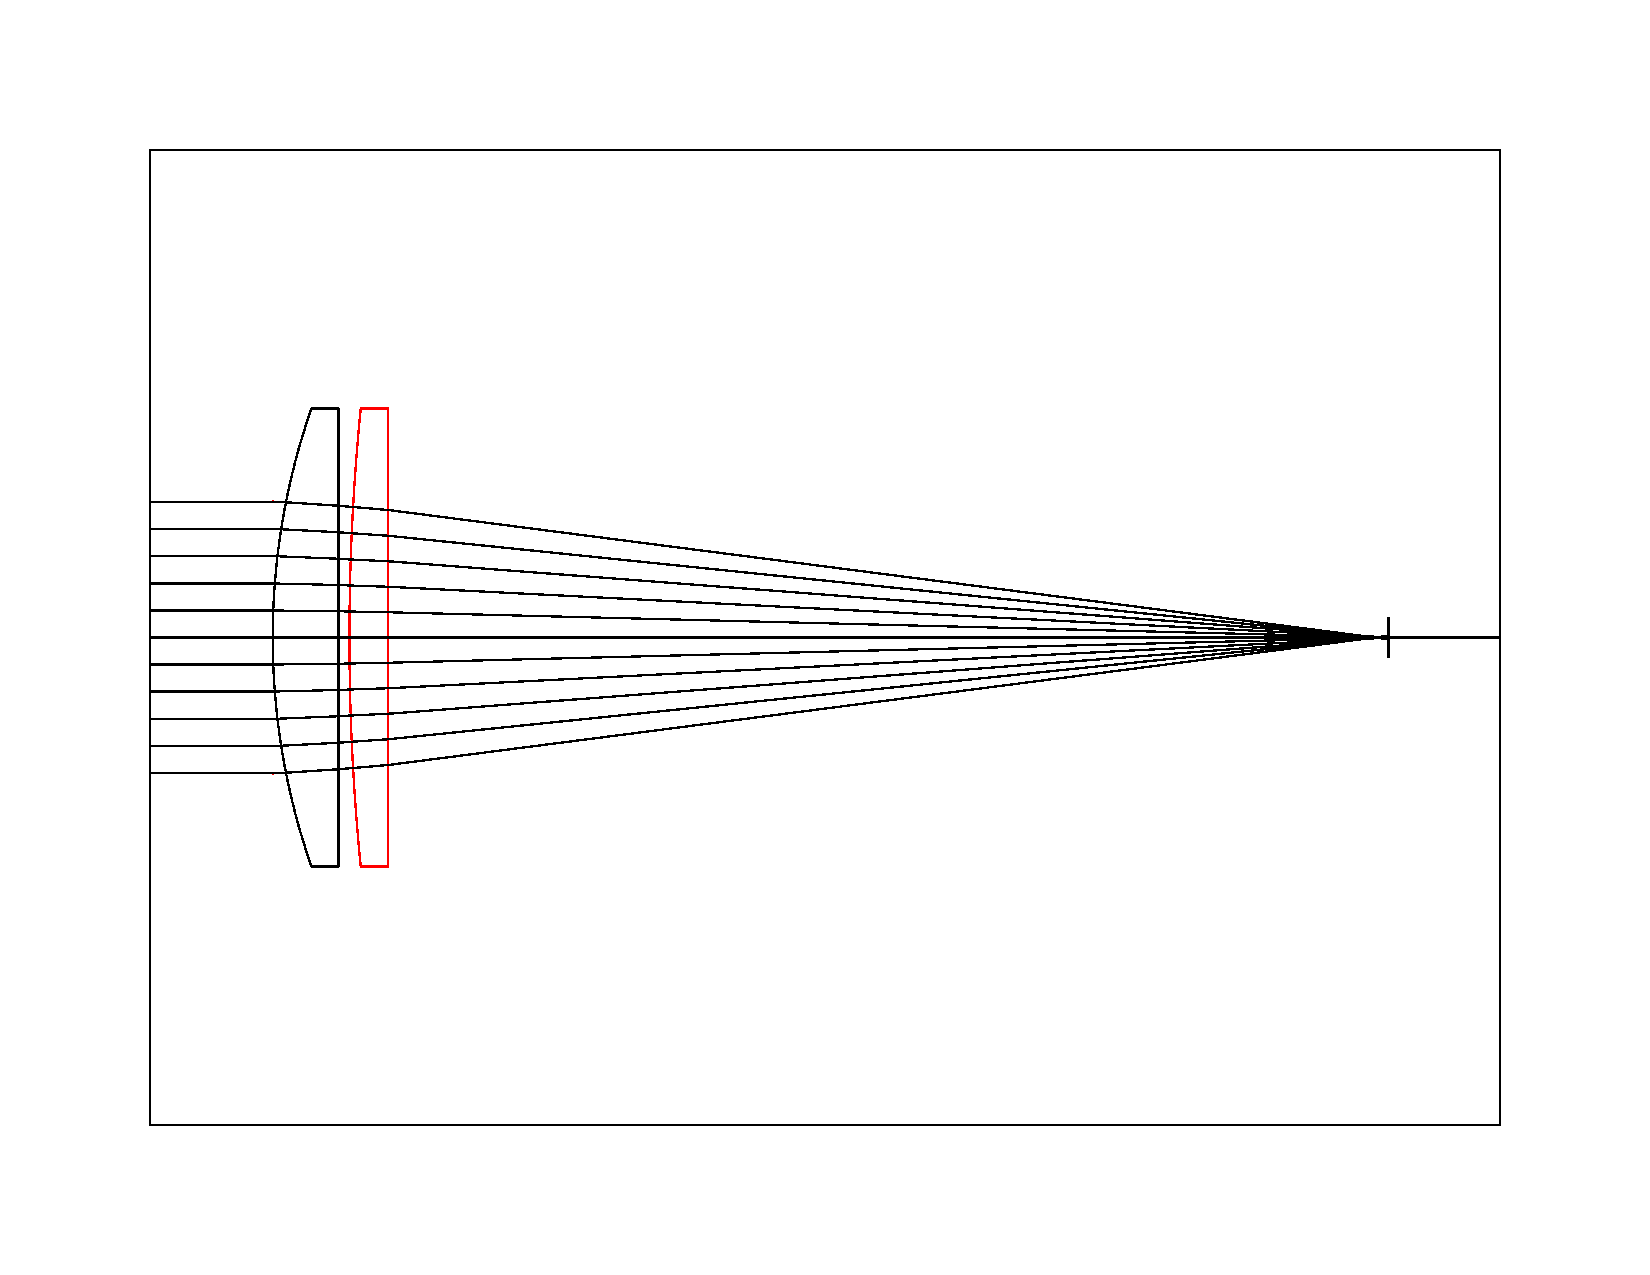
\includegraphics[width=\textwidth]{assets/4 experiments/500 and 150 lenses.pdf}
                    \caption{Multi-lens system}
                \end{figure}
    
    
                \begin{figure}[!ht]
                    \centering
                    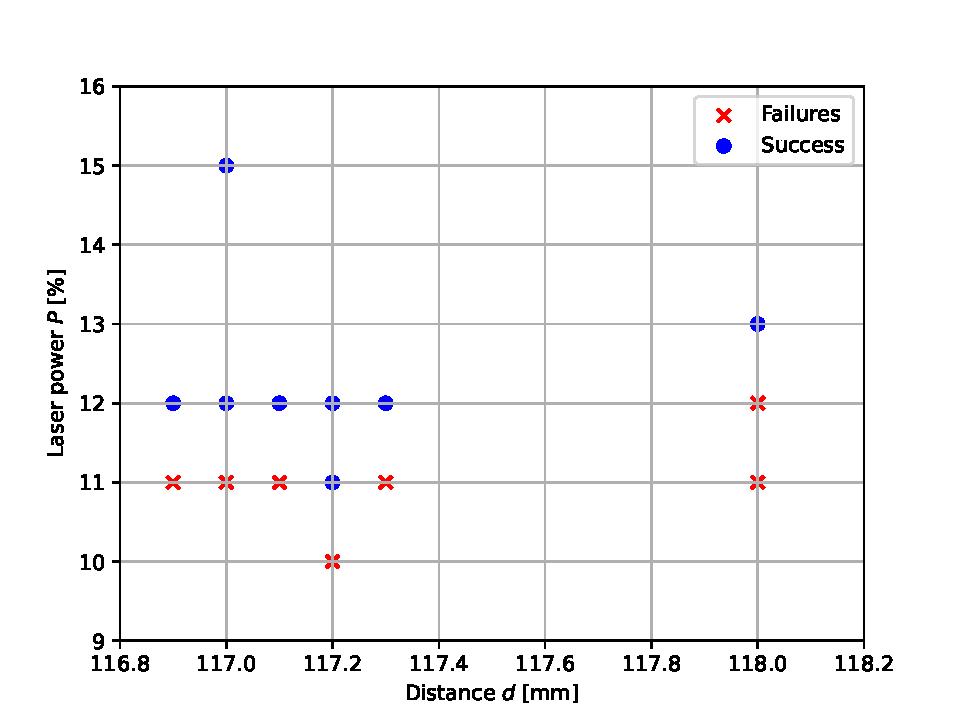
\includegraphics[width=0.75\textwidth]{assets/4 experiments/duallens_focus_threshold.pdf}
                    \caption{Multi-lens system}
                \end{figure}
    
                % Section on power meter reading lower pulsed power at these low power settings, like about 200W
    
                The completion of these tests validated LSP generation in the CW power regime of the laser. The V2 thruster was then set up to test CW operation with flowing argon.
            
            \section{V2 Bringing the pulsed power down, again}
            
                To prevent the damage to the thruster seen previously, a rear window mount was manufactured. This allows the laser energy that is not absorbed to pass freely through the apparatus, also enabling power meter measurements. 
                
                % Photo of rear window mount and damaged window
    
                As can be seen above, the window suffered laser damage after this round of testing. However, this damage proved minor as the window was used to align the laser focus with the spark gap, not to measure power absorption.
                
                The following figure presents the LSP initiation attempts with focus distance, similarly to the graphs presented in \autoref{sec:pulse_power_down_V1}.
    
                \begin{figure}[!ht]
                    \centering
                    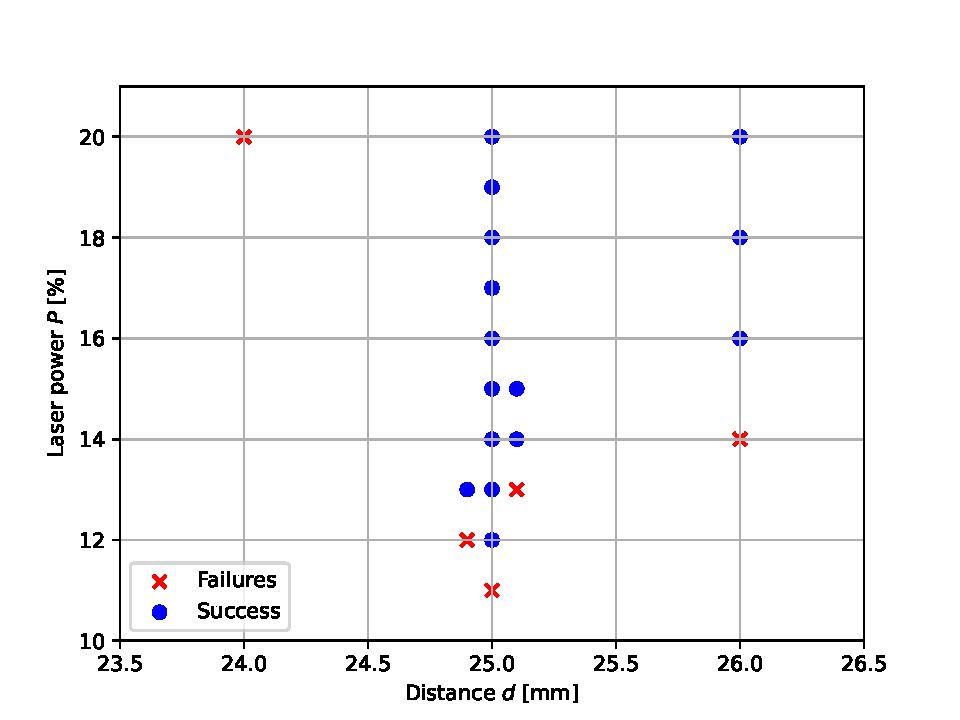
\includegraphics[width=0.75\textwidth]{assets/4 experiments/V2_focus_threshold.pdf}
                    \caption{LSP threshold graph for V2}
                \end{figure}
    
                The real amount of power in the pulsed shots was also measured to validate the \qty{11}{\%} threshold quoted previously. 10 shots each at \qtylist{10; 12}{\%} were measured with the power meter, with statistics compiled by the power meter software (see \autoref{label})
    
                \begin{table}[!ht]
                    \caption{Statistics from the power meter after 10 times \qty{50}{ms} laser shots at \qty{10}{\%} and \qty{12}{\%} power}
                    \label{tab:laser shot statistics}
                    \begin{tabular}{lll}
                    \textbf{Value {[}Unit{]}} & \textbf{10x 50 ms shots at 10\% power} & \textbf{10x 50 ms shots at 12\% power} \\ \hline
                    Average value {[}J{]}  & 9.985 & 12.89 \\
                    Maximum value {[}J{]}  & 10.2  & 13.3  \\
                    Minimum value {[}J{]}  & 9.63  & 12.0  \\
                    RMS Stability {[}\%{]} & 1.690 & 2.811 \\
                    PTP Stability {[}\%{]} & 5.599 & 10.31 \\
                    Average power {[}W{]}  & 0.490 & 1.14  \\
                    Std deviation {[}J{]}  & 0.169 & 0.362 \\ \hline
                    \end{tabular}
                \end{table}
                
                At 10\% power, an 9.985 J average during \qty{50}{ms} gives an average power of \qty{200}{W}, lower than the expected \qty{300}{W} For \qty{12}{\%}. This revealed a higher power threshold, in terms of percentage, than previously thought. Extrapolating from these measurements, \qty{300}{W} is achieved at \qty{13.5}{\%}. This validated that the

            \section{New nozzle design}

                Attempts at pulsed LSP ignition with the original nozzle gave 
                
                \begin{figure}[!ht]
                    \centering
                    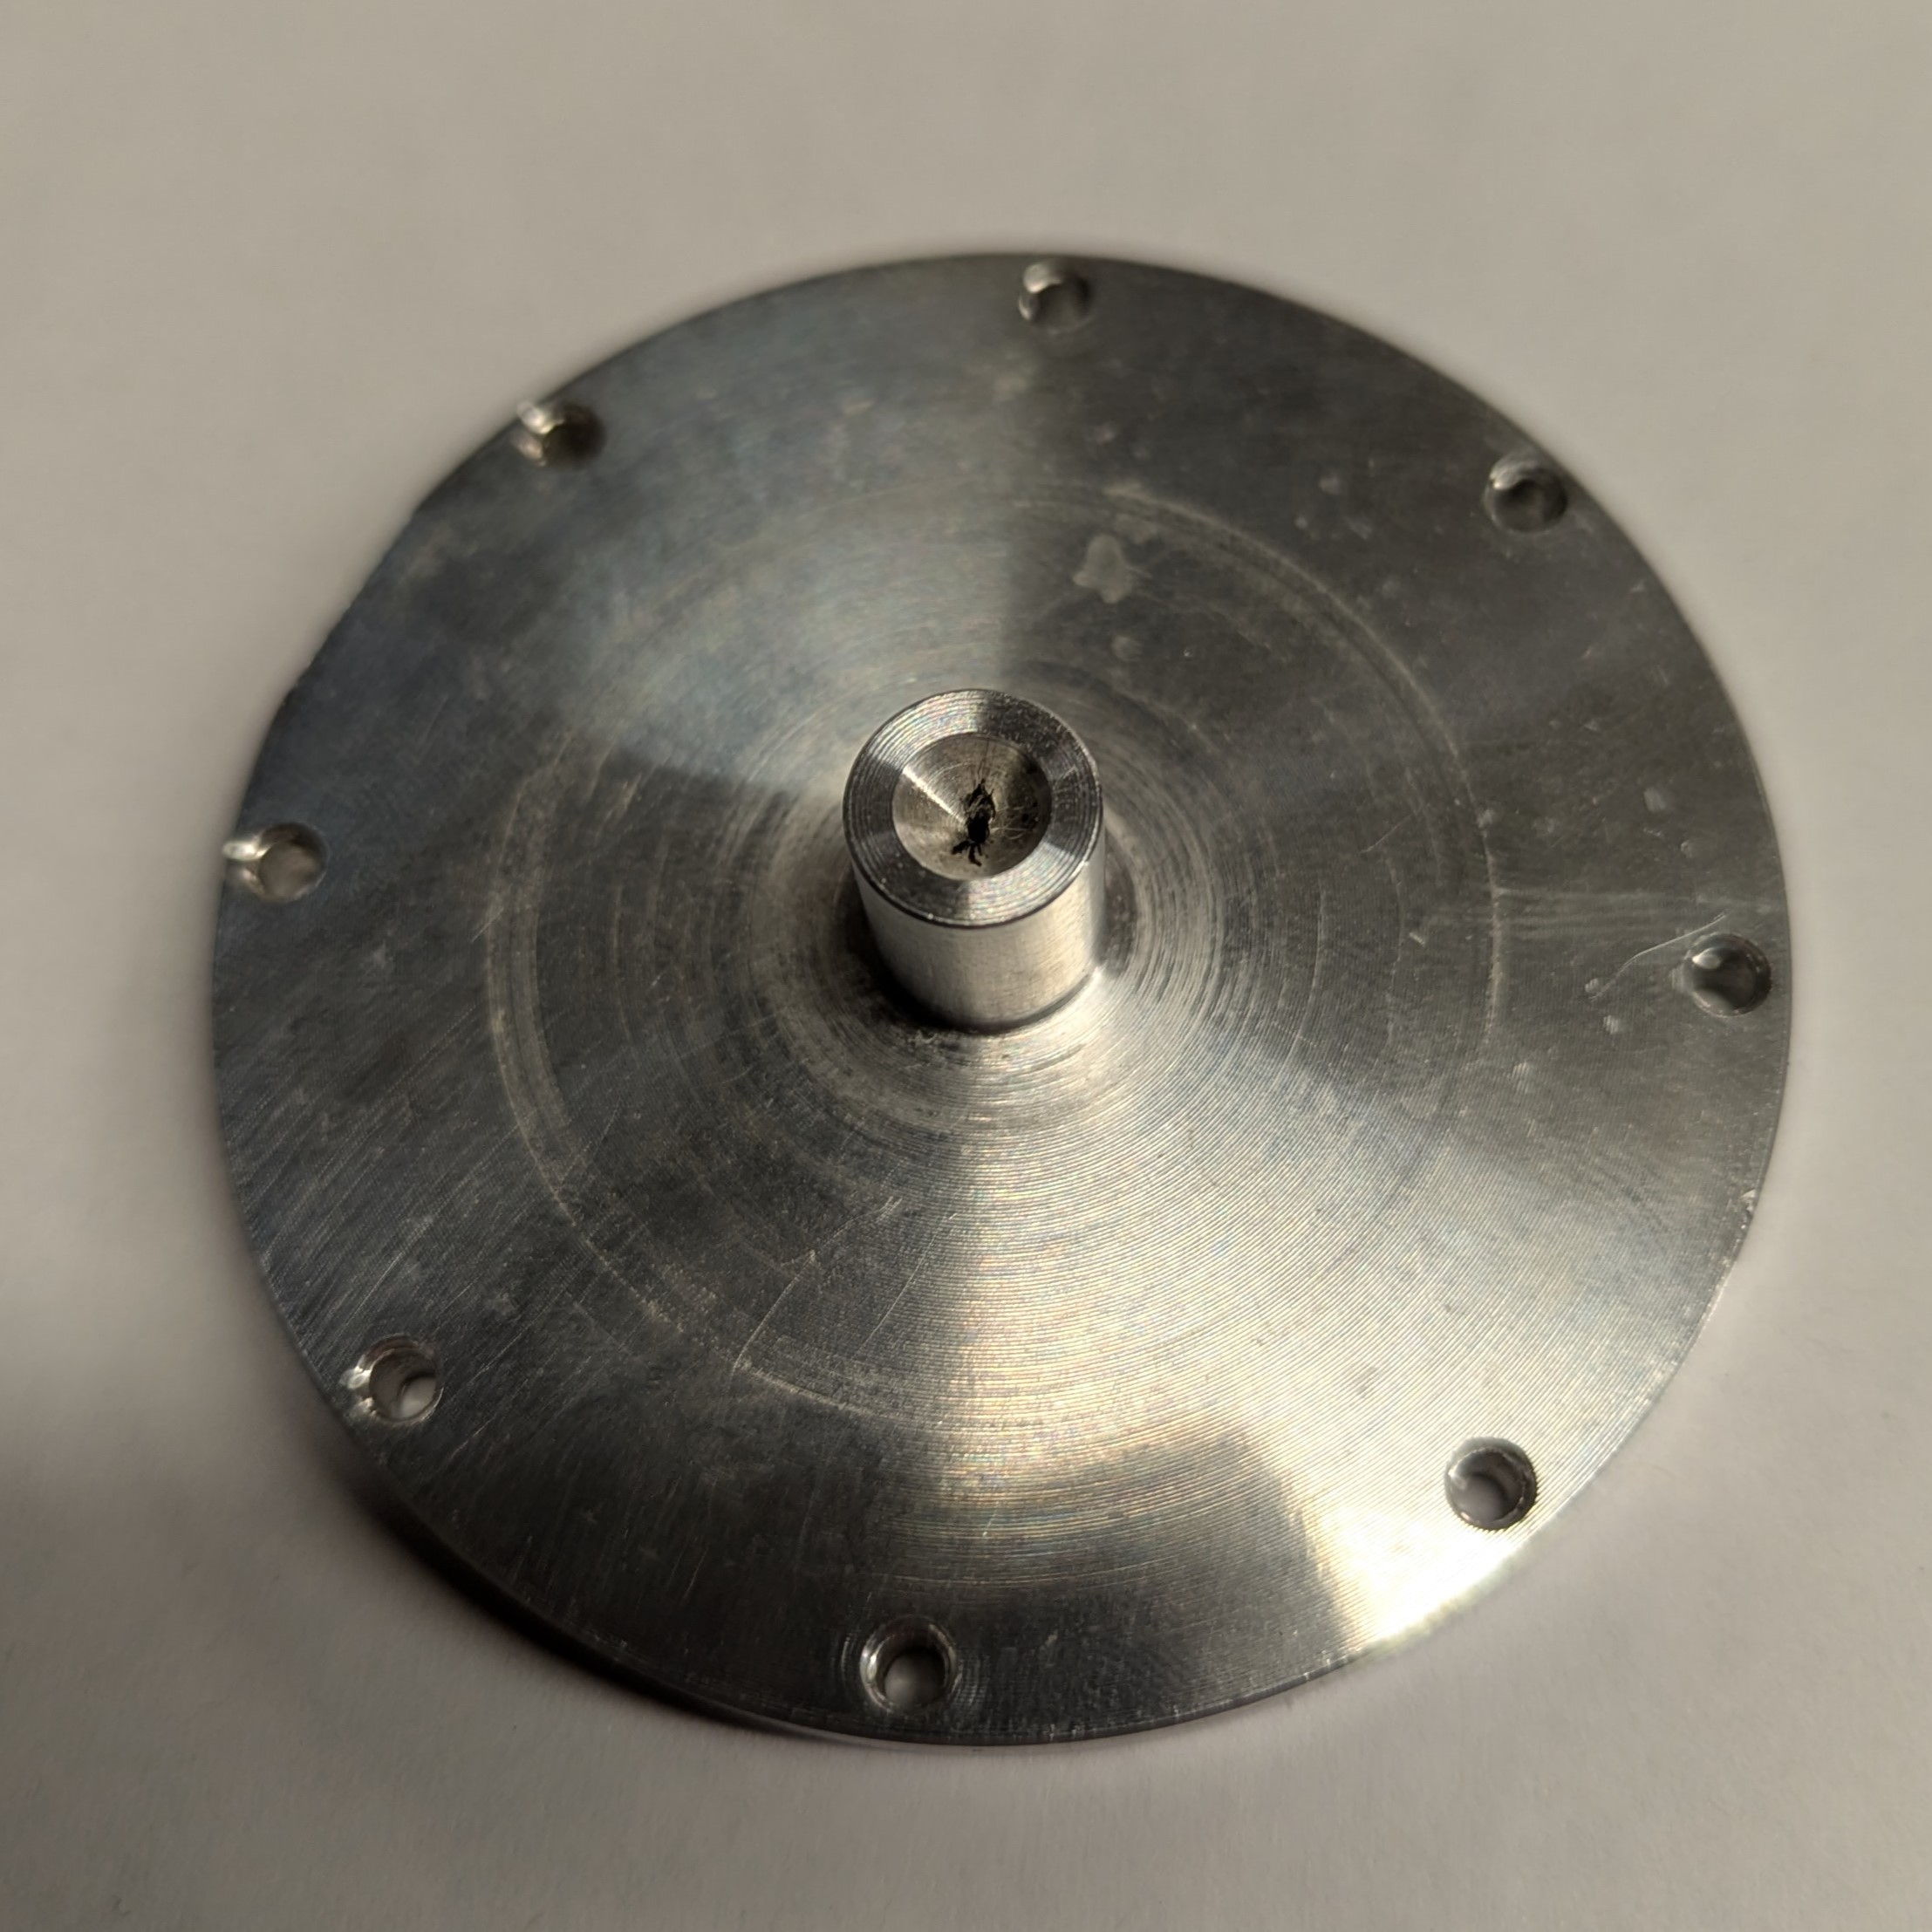
\includegraphics[width=0.5\textwidth]{assets/4 experiments/Nozzle damage.jpg}
                    \caption{Nozzle laser damage}
                \end{figure}
            
                To solve the ablation of the aluminum nozzle under pulsed laser shots, the V2 thruster inner cylinder was modified, and a new backplate was manufactured to accept graphite nozzle inserts. These inexpensive, changeable inserts are made from superfine iso-molded graphite rods sourced from Graphitestore (0.500" diameter x 12"L, SKU GT001685).
    
                [image of drawing highlighting changes]

    \section{Cold flow test friction HYSTERESIS}

                [FRICTION HYSTERESIS PROBLEMS: TO DISCUSSION] To correct these problems, a more sensitive load cell was installed with a \qtyrange{0}{5}{N} force sensing range (Honeywell FSG005WNPB). However, the issue remained.

            A different type of thrust stand (e.g. a rotating arm), could eventually be built to measure thrust in a more repeatable manner.